\documentclass[12pt]{article}
 \usepackage[margin=1in]{geometry} 
\usepackage{amsmath,amsthm,amssymb,amsfonts}
\usepackage{graphicx}
\usepackage{array}
\newcolumntype{P}[1]{>{\centering\arraybackslash}p{#1}}
\newcommand{\N}{\mathbb{N}}
\newcommand{\Z}{\mathbb{Z}}
 \usepackage{media9}
 \usepackage{hyperref}
\newenvironment{problem}[2][Problem]{\begin{trivlist}
\item[\hskip \labelsep {\bfseries #1}\hskip \labelsep {\bfseries #2.}]}{\end{trivlist}}
%If you want to title your bold things something different just make another thing exactly like this but replace "problem" with the name of the thing you want, like theorem or lemma or whatever
 
\begin{document}
 
%\renewcommand{\qedsymbol}{\filledbox}
%Good resources for looking up how to do stuff:
%Binary operators: http://www.access2science.com/latex/Binary.html
%General help: http://en.wikibooks.org/wiki/LaTeX/Mathematics
%Or just google stuff
 
\title{Homework-5 \\ 3D Optical Character Recognition using Neural networks}
\author{N Dinesh Reddy \\ dnarapur@andrew.cmu.edu }

\newpage

\maketitle

\section{Theory}

\begin{problem}{1.1}
\end{problem}
\begin{problem}{1.4}

\end{problem}
\newpage
\section{}

\begin{problem}{2.1}
\end{problem}

\begin{problem}{2.2}
\end{problem}

\begin{problem}{2X}
\end{problem}

\begin{problem}{2.3}

\end{problem}
\begin{problem}{2.4}
\end{problem}
\begin{problem}{2.5}
\end{problem} 

\begin{problem}{3.1.2}
The four plots for the training are displayed with different learning rate are shown below:\\
For Learning Rate 0.001:\\
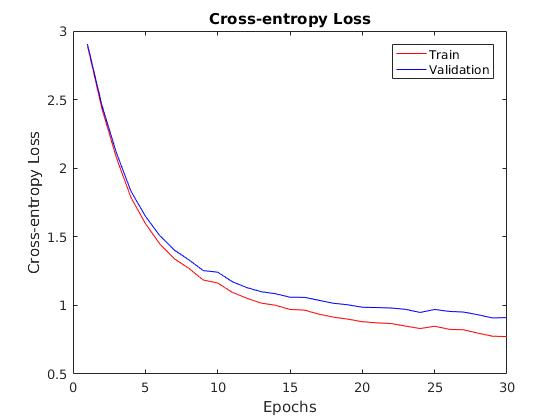
\includegraphics[scale=0.4]{images/learning_acc_0_001.jpg} \ 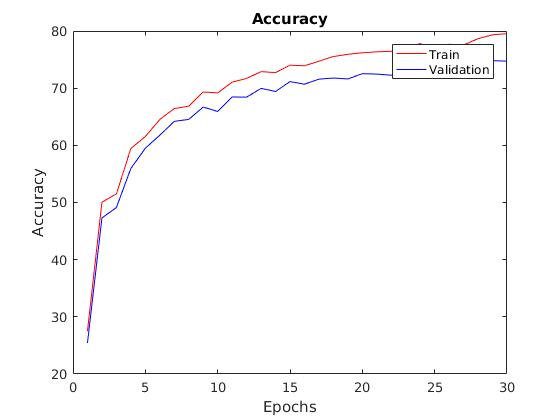
\includegraphics[scale=0.4]{images/learning_cross_0_001.jpg} \\
For Learning Rate 0.01:\\
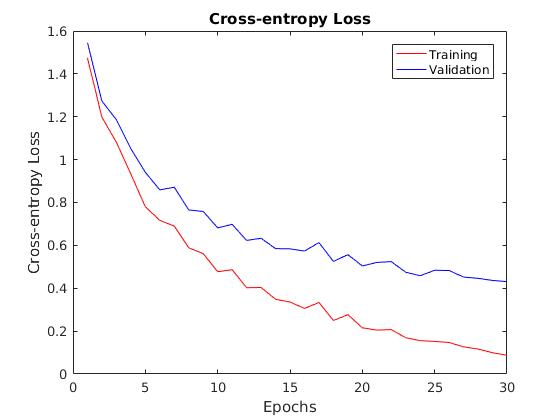
\includegraphics[scale=0.4]{images/learning_cross_0_01.jpg}\
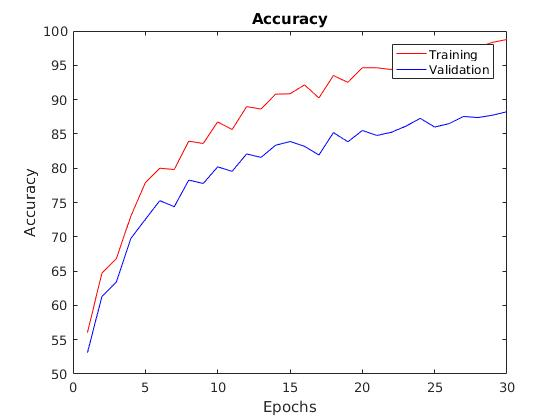
\includegraphics[scale=0.4]{images/learning_acc_0_01.jpg}   \\

The learning rate with 0.01 shows a better accuracy on the training and validation set this can be attributed to the fact that higher learning rate causes the weights to change rapidly to give better accuracy with lesser number of epochs. but the lower learning rate shows a lesser variation in the accuracy between the training and the validation accuracies. The test accuracy for the model with learning rate 0.01 is {\bf 89.3077} and the loss is {\bf 0.4464}.
\end{problem}


\begin{problem}{2.7}

\end{problem}
\newpage
\begin{problem}{QX}
\end{problem}

\end{document}